\documentclass[12pt,a4paper]{report}
\usepackage[affil-it]{authblk}
% Packages
\usepackage[utf8]{inputenc}
\usepackage{dirtree}
\usepackage{amsmath}
\usepackage{amssymb}
\usepackage{graphicx}
\usepackage{hyperref}
\usepackage{cleveref}
\usepackage{geometry}
\usepackage{enumitem}
\usepackage{booktabs}

\geometry{a4paper, margin=1in}

% Title Page
\title{Dysruption - Action Analysis}
\author{Rishitosh Kumar Singh}
\affil{Arizona State University}

\date{\today}

\begin{document}

\maketitle
\tableofcontents
\clearpage

\chapter{Introduction}
\label{chap:introduction}
    This report presents the work conducted over the semester on a project focused on analyzing decision-making strategies within critical infrastructure networks through interactive simulation games. The primary objective was to design and develop autonomous bots capable of playing two online strategy games—\textit{Break it Bad} and \textit{Save Our System (Scenario 1)}—and to evaluate their performance by recording and analyzing their actions and corresponding scores.

    \begin{figure}[h!]
        \centering
        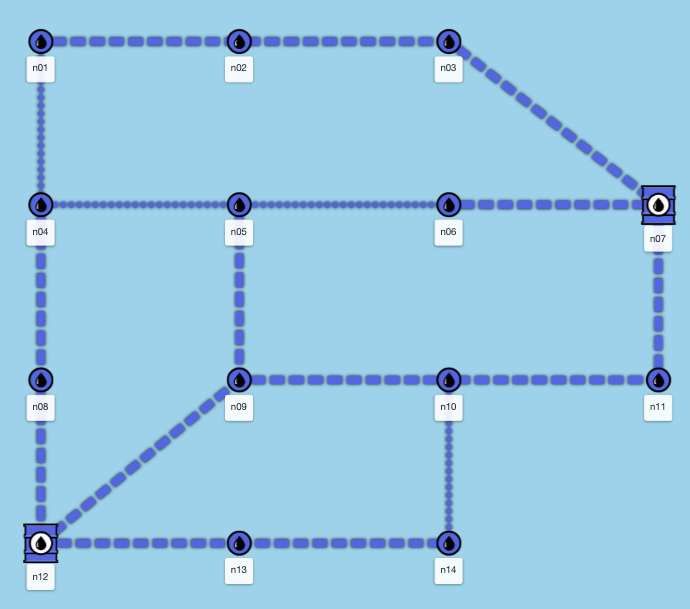
\includegraphics[width=0.6\textwidth]{images/game-graph.png}
        \caption{Game network with two supply nodes, and 12 demand nodes with "has flow", "no flow" edges.}
        \label{fig:game-graph}
    \end{figure}

    Both games simulate a fuel transportation network composed of supply nodes, demand nodes, and connecting pipelines. In \textit{Break it Bad}, the objective is to disrupt the network as effectively as possible using a limited number of actions. Success is measured by the cost inflicted on the system through strategically damaging pipelines and cutting off supply routes. In contrast, \textit{Save Our System} challenges players to maintain network stability in the face of potential disasters. The objective in this game is to mitigate risk, prepare for unpredictable events, and ensure uninterrupted fuel flow at minimal cost

    The project aimed to:
    \begin{itemize}
        \item Develop autonomous bots to play both games using rule-based strategies.
        \item Record the sequence of actions taken and the resulting scores.
        \item Analyze how different types of actions influence system performance under various conditions.
    \end{itemize}

    To accomplish these objectives, object-oriented programming principles were applied to structure the bots, ensuring modularity, extensibility, and ease of testing. Additionally, a logging system was developed to capture data from each gameplay session. This report outlines the design process, implementation logic, analysis methods, and the insights gained through experiments with different bot strategies.

\chapter{Game and Bot Framework}
\label{chap:game-bot-framework}
    There are a total of $10$ games available for users to play, but this semester the focus was on two of them, as discussed in \cref{chap:introduction}. To ensure that the project and modular bot framework are extensible, the codebase was designed to accommodate various strategies and gameplay logic. The project is structured around a base class, \texttt{DysruptionGame}, which encapsulates shared functionalities such as browser login, map interaction, state inspection, and common game utilities. This base class is further extended by two specialized subclasses: \texttt{BreakItBad} and \texttt{SaveOurSystem}, each implementing game-specific strategies. This design facilitates easy swapping of strategies and analysis of performance data across multiple simulation runs, while also enabling the addition of new games in the future for analysis. More details are provided in \cref{sec:appendix-bot-framework}.

    \begin{figure}[h!]
        \centering
        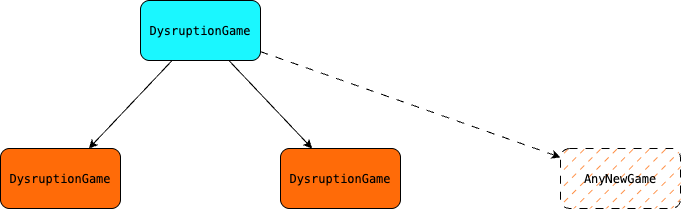
\includegraphics[width=0.8\textwidth]{images/class.png}
        \caption{Class diagram illustrating the inheritance structure of the bot framework. Any new game can be added by extending the \texttt{DysruptionGame} class.}
        \label{fig:class-diagram}
    \end{figure}

    \section{Bot Action Logics}
    \label{sec:bot-action-logics}
        For each game, the bot was designed with a set of action logics to choose from. The bot can be configured with various decision logics, referred to as “intelligence levels,” which differ for each game. These intelligence levels are outlined as follows:
        
        \begin{itemize}
            \item \textbf{Break It Bad}:
            \begin{itemize}
                \item \textbf{not\_dumb}: Acts similarly to a typical user, although the bot does not have the ability to determine which action will yield the highest score.
                \item \textbf{dumb}: Takes actions without considering their effectiveness, including moves that a regular user would typically avoid, resulting in no improvement in score.
            \end{itemize}
            
            \item \textbf{Save Our System}:
            \begin{itemize}
                \item \textbf{only\_maintain}: Always performs the maintain action on the selected edge if the bot randomly decides to act.
                \item \textbf{only\_replace}: Always performs the replace action on the selected edge if the bot randomly decides to act.
                \item \textbf{only\_repair}: Always performs the repair action on the selected edge if the bot randomly decides to act.
                \item \textbf{weighted\_random}: Chooses an action based on the condition of the edge (FCI) and the available budget:
                \begin{itemize}
                    \item If the FCI $\geq 99.6$ and the cost of maintenance is within the budget, performs the maintain action.
                    \textit{(Rationale: At this level, the pipeline is nearly perfect, so maintaining it helps prolong its optimal condition, preventing future degradation.)}

                    \item If $ 92 \leq$ FCI $< 99.6$ and the cost of repair is within the budget, performs the repair action.
                    \textit{(Rationale: This range indicates that the pipeline is functioning but showing signs of wear. Repairs can restore it to a more robust state without incurring the high costs of replacement.)}

                    \item If FCI $< 92$ and the cost of replacement is within the budget, performs the replace action.
                    \textit{(Rationale: A low FCI suggests significant wear or damage. Replacing the pipeline ensures long-term reliability, especially when incremental repairs are not sufficient.)}

                \end{itemize} 
            \end{itemize}
        \end{itemize}  

        The bot’s decision-making process, as illustrated in \cref{fig:bot-logic}, is structured as a series of logical steps that guide its actions during gameplay. The flowchart provides a clear visual representation of how the bot evaluates the game state, selects an action, and executes it.

        \begin{figure}[!htbp]
            \centering
            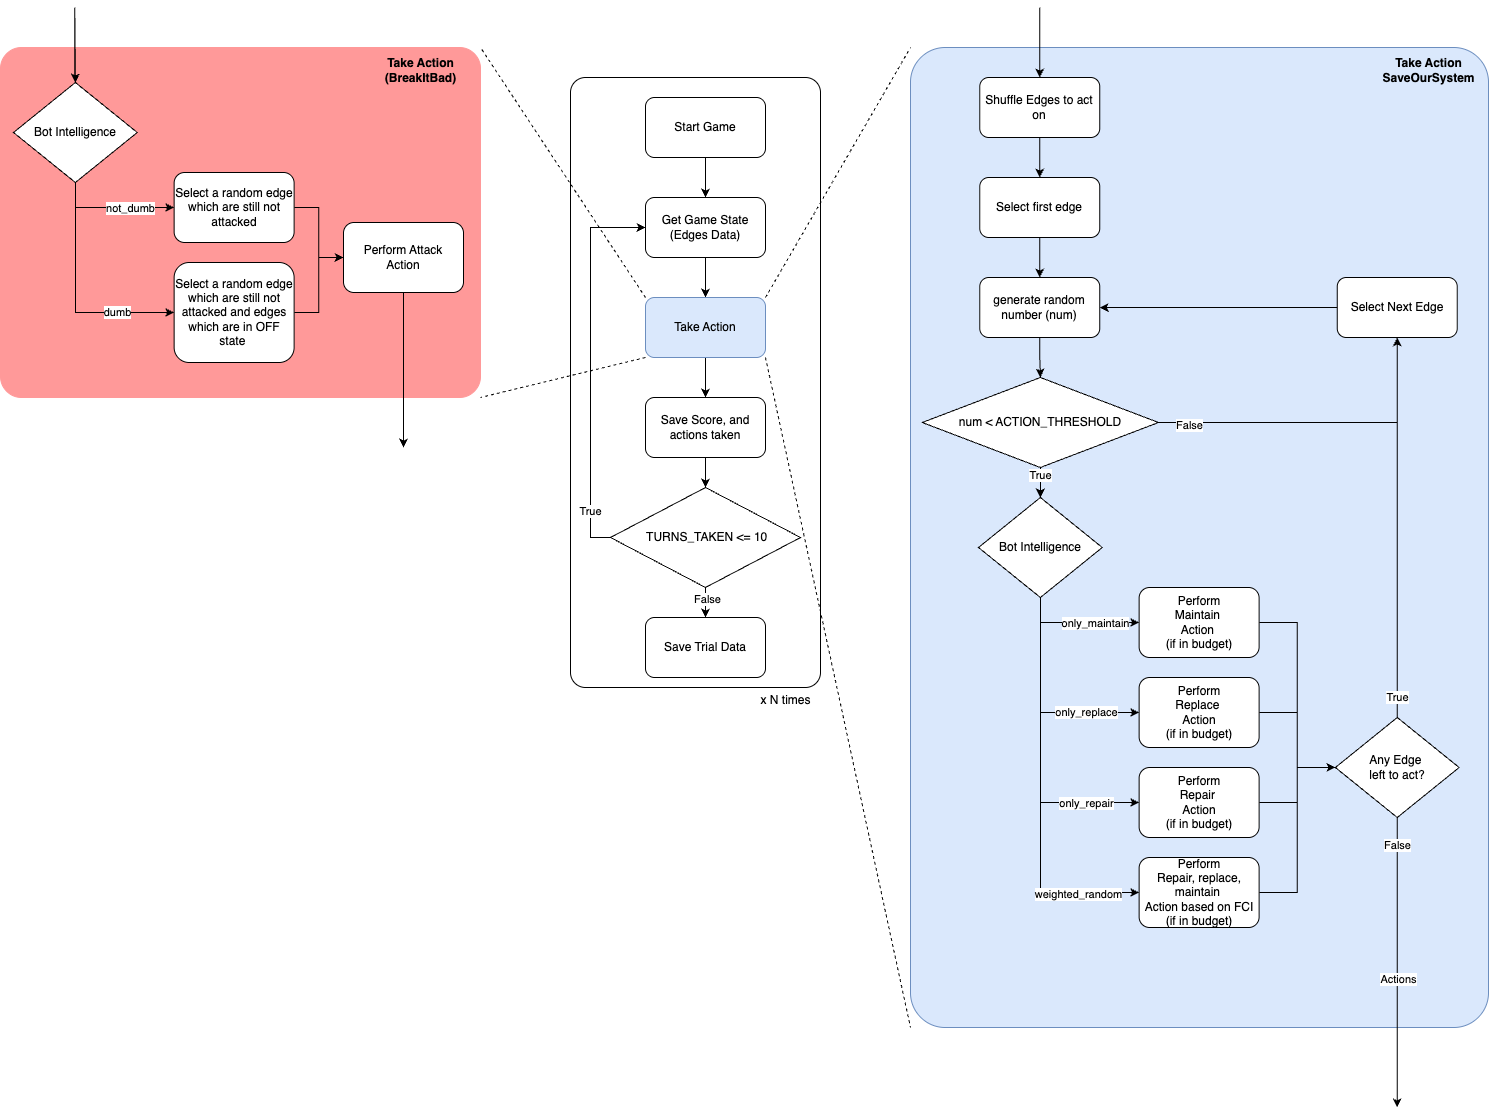
\includegraphics[width=0.8\textheight, angle=90]{images/bot-logic.png}
            \caption{Flowchart illustrating the decision-making logic of the bots for both games. The central white box is implemented in the \texttt{bot.py} and \texttt{bot-savepursystem.py} files, while the other two boxes are implemented within their respective game classes in \texttt{src/game.py}.}
            \label{fig:bot-logic}
        \end{figure}

    \chapter{Result and Analysis}
    \label{chap:score-analysis}
        \section{Break It Bad}

        To evaluate the performance of the bot in the \textit{Break It Bad} game, the bot was run in \texttt{not\_dumb} intelligence mode for approximately 500 game simulations. In each simulation, the bot performed up to 5 moves, and the resulting score was recorded after each move. The objective was to analyze the progression of scores with each action and to identify the move sequences that resulted in the highest disruption scores.

        \begin{figure}[h!]
            \centering
            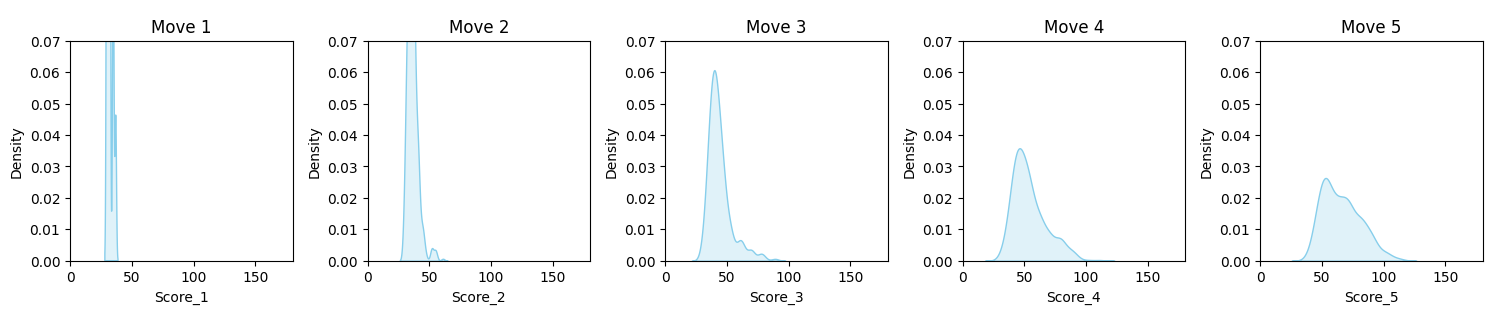
\includegraphics[width=\textwidth]{images/kde-breakitbad.png}
            \caption{KDE plot showing the distribution of scores after each move over 500 simulations (maximum of 5 moves shown). Higher density towards the right indicates increasing score trends.}
            \label{fig:kde-breakitbad}
        \end{figure}

        As shown in \cref{fig:kde-breakitbad}, the KDE plots illustrate how the score distribution changes with each move. Initially, the scores are tightly concentrated, but as the game progresses, the distributions broaden and shift toward higher values, indicating increasing disruption. By Move 4 and Move 5, the distributions become significantly wider and start to exhibit bi-modal characteristics.

        To gain deeper insights into the bot’s decision-making process, the sequence of moves leading to the highest score after 5 moves was extracted. The maximum score achieved was \textbf{113}. The corresponding move sequence is presented in \cref{tab:breakitbad-moves}, where each entry represents an edge that was attacked during the game. The edges are denoted as pairs of nodes, indicating the targeted connections.

        \begin{table}[h!]
            \centering
            \begin{tabular}{cc}
            \toprule
            \textbf{Move} & \textbf{Edge Attacked} \\
            \midrule
            1 & \texttt{7 <-> 3} \\
            2 & \texttt{12 <-> 8} \\
            3 & \texttt{7 <-> 6} \\
            4 & \texttt{11 <-> 7} \\
            5 & \texttt{5 <-> 9} \\
            \bottomrule
            \end{tabular}
            \caption{Sequence of moves leading to the highest score in \textit{Break It Bad}. Each entry \texttt{x <-> y} represents an attack on the pipeline (edge) connecting node \texttt{x} to node \texttt{y}.}
            \label{tab:breakitbad-moves}
        \end{table}
            
        % These results highlight that specific combinations of edges consistently result in greater disruption, offering insights into the network’s most vulnerable points when targeted early.
            
        \section{Save Our System}

        To assess different bot strategies in the \textit{Save Our System} game, all four intelligence levels from \cref{sec:bot-action-logics} were tested, with approximately $20-30$ trials conducted for each strategy. The bot’s actions and resulting scores were recorded after each game step. The best scores for each strategy are summarized in \cref{tab:strategy-comparison}. The results from all scenarios were then aggregated and analyzed to determine the best-performing strategy based on the highest final score achieved.

        \begin{table}[h!]
            \centering
            \begin{tabular}{lc}
            \toprule
            \textbf{Strategy} & \textbf{Max Score Achieved} \\
            \midrule
            only\_maintain & 19 \\
            only\_repair & 15 \\
            only\_replace & 20 \\
            \textbf{weighted\_random} & \textbf{28} \\
            \bottomrule
            \end{tabular}
            \caption{Summary of the maximum scores achieved by different strategies in the \textit{Save Our System} game.}
            \label{tab:strategy-comparison}
        \end{table}
            
            % These results indicate that the \textbf{weighted_random} strategy consistently outperforms the other strategies, achieving the highest maximum score. This suggests that dynamically adjusting actions based on edge conditions and budget availability is more effective compared to using a fixed action strategy.

        \begin{table}[h!]
            \centering
            \begin{tabular}{ccp{12cm}}
            \toprule
            \textbf{Move} & \textbf{Score} & \textbf{Actions Taken} \\
            \midrule
            1 & 3 & MAINTAIN: 10\texttt{$\leftrightarrow$}11, 7\texttt{$\leftrightarrow$}6, 10\texttt{$\leftrightarrow$}14, 14\texttt{$\leftrightarrow$}13, 2\texttt{$\leftrightarrow$}1 \\
            2 & 6 & MAINTAIN: 4\texttt{$\leftrightarrow$}1, 11\texttt{$\leftrightarrow$}7, 7\texttt{$\leftrightarrow$}6 \\
            3 & 9 & MAINTAIN: 14\texttt{$\leftrightarrow$}13, 12\texttt{$\leftrightarrow$}8, 9\texttt{$\leftrightarrow$}12, 2\texttt{$\leftrightarrow$}1, 11\texttt{$\leftrightarrow$}7 \\
            4 & 12 & REPAIR: 9\texttt{$\leftrightarrow$}10, REPLACE: 2\texttt{$\leftrightarrow$}3, MAINTAIN: 2\texttt{$\leftrightarrow$}1, REPAIR: 5\texttt{$\leftrightarrow$}9, MAINTAIN: 14\texttt{$\leftrightarrow$}13 \\
            5 & 15 & REPAIR: 6\texttt{$\leftrightarrow$}5, MAINTAIN: 11\texttt{$\leftrightarrow$}7, REPLACE: 4\texttt{$\leftrightarrow$}5 \\
            6 & 18 & REPAIR: 5\texttt{$\leftrightarrow$}9, REPAIR: 10\texttt{$\leftrightarrow$}14, MAINTAIN: 11\texttt{$\leftrightarrow$}7 \\
            7 & 21 & REPAIR: 12\texttt{$\leftrightarrow$}8, REPAIR: 9\texttt{$\leftrightarrow$}12, REPAIR: 13\texttt{$\leftrightarrow$}12 \\
            8 & 24 & REPAIR: 7\texttt{$\leftrightarrow$}3, REPAIR: 9\texttt{$\leftrightarrow$}12, REPAIR: 2\texttt{$\leftrightarrow$}3, REPAIR: 10\texttt{$\leftrightarrow$}14, REPAIR: 10\texttt{$\leftrightarrow$}11 \\
            9 & 27 & REPLACE: 14\texttt{$\leftrightarrow$}13, REPAIR: 7\texttt{$\leftrightarrow$}6, REPAIR: 11\texttt{$\leftrightarrow$}7, REPAIR: 13\texttt{$\leftrightarrow$}12 \\
            10 & 28 & REPLACE: 4\texttt{$\leftrightarrow$}5, REPAIR: 4\texttt{$\leftrightarrow$}1, REPAIR: 10\texttt{$\leftrightarrow$}11, REPAIR: 11\texttt{$\leftrightarrow$}7 \\
            \bottomrule
            \end{tabular}
            \caption{Score progression of the best trial for the \textit{Save Our System} game. The table displays the score after each move and the corresponding actions taken. The actions are categorized as MAINTAIN, REPAIR, or REPLACE. Each entry \texttt{x <-> y} represents an action performed on the pipeline (edge) connecting node \texttt{x} to node \texttt{y}.}
            \label{tab:score-progression}
        \end{table}

        \Cref{tab:score-progression} highlights how the best move sequence in the \texttt{weighted\_random} strategy, in which the bot dynamically chooses actions based on the Failure Condition Index (FCI) of each pipeline segment and the available budget. This strategy outperformed other fixed-action methods, achieving a maximum score of $28$. The success of this approach lies in its ability to balance maintenance, repair, and replacement actions according to the pipeline’s condition.

        The effectiveness of the weighted random strategy can be attributed to its adaptive nature. By continuously assessing the condition of each pipeline and weighing the costs of potential actions, the bot optimizes resource allocation. This balanced approach is crucial in managing critical infrastructure, where maintaining optimal performance with limited resources is a constant challenge.

        In the early game (moves 1-3), the bot primarily performed maintenance actions to preserve high-FCI pipelines, preventing premature deterioration and ensuring cost-effective long-term stability. As the game progressed (moves 4-7), the bot adapted by prioritizing repairs when FCI dropped below $99.6$, effectively restoring moderately degraded pipelines without incurring replacement costs. In the late game (moves 8-10), the bot focused on replacing severely degraded pipelines (FCI $< 92$) when repairs became inefficient, ensuring that critical failures were addressed in a budget-optimized manner.

    \chapter{Conclusion and Future Work}
    \label{chap:conclusion-future-work}
        
        In conclusion, the project provided a valuable learning experience, resulting in the development of a modular bot framework that can be extended to incorporate additional games in the future if needed. For this semester, the development of the bots for the \textit{Break It Bad} and \textit{Save Our System} games was completed successfully, with both bots functioning as expected. The bots demonstrated the ability to play the games using different strategies and intelligence levels as specified in the project requirements.
        
        For future work, the \textit{Save Our System} game bot can be further enhanced by incorporating reinforcement learning (RL) to improve decision-making. Instead of predefining strategies such as “only\_maintain” or “only\_replace,” the bot could autonomously learn optimal moves through continuous gameplay. Using RL, the bot would explore various actions, and after each iteration, it would learn which moves yield the best rewards. After several hundred iterations, the bot would develop a robust policy to optimize gameplay, eliminating the need for manually defining strategies and allowing the bot to adapt to the game’s random environment.
        
        Since the project follows a modular architecture, developing an RL-based bot for the \textit{Save Our System} game would be relatively straightforward. The bot framework’s extensible design allows for the seamless integration of new games and strategies, enabling further exploration of advanced decision-making algorithms in future projects.


    \chapter{Acknowledgements}
    \label{chap:acknowledgements}
        
        The author would like to express gratitude to Dr. Thomas Seager for providing the opportunity to contribute to his research project. His guidance and insights were instrumental in shaping the direction of the work and ensuring its successful completion. Appreciation is also extended to Mazin Abdel Magid for providing detailed walkthroughs of the project and its requirements, which greatly facilitated the development process.

    \clearpage

\appendix
    \chapter{Repository Structure}

    This chapter provides an overview of the repository structure along with a brief description of each file and folder. It also includes guidelines on how to use the repository and where to make changes if needed.
    \dirtree{%
        .1 /.
        .2 config.
        .3 breakitbad.py.
        .3 saveoursystem1.py.
        .2 src.
        .3 game.py.
        .3 utils.
        .4 const.py.
        .4 Edge.py.
        .4 metrics.py.
        .4 Node.py.
        .2 bot.py.
        .2 bot-saveoursystem.py.
        .2 requirements.txt.
    }

    \vspace{1cm}
    The details of the files and folders are as follows:

    \begin{itemize}
        \item \textbf{config/}: Contains configuration files for each game that the bot reads. These files include settings necessary for the bot’s operation. Each game has its own configuration file, allowing users to adjust parameters such as the number of trials, the game URL, and the bot’s intelligence level.
        \begin{itemize}
            \item \texttt{break\_it\_bad.py}: Configuration file for the \texttt{BreakItBad} game.
            \item \texttt{save\_our\_system.py}: Configuration file for the \texttt{SaveOurSystem} game.
        \end{itemize}
        \item \textbf{src/}: Contains the source code for the bot framework and game-specific implementations.
        \begin{itemize}
            \item \texttt{game.py}: The main game file where the base game class and the derived classes (\texttt{BreakItBad} and \texttt{SaveOurSystem}) are defined. New games can be added by defining them in this file.
            \item \texttt{utils/}: Contains utility files such as data classes for storing node and edge data, as well as constants used within the games.
        \end{itemize}
        \item \textbf{bot.py}: The bot script for the \texttt{BreakItBad} game. To run the bot, execute the command \texttt{python3 bot.py} in the terminal.
        \item \textbf{bot-saveoursystem.py}: The bot script for the \texttt{SaveOurSystem} game. To run the bot, execute the command \texttt{python3 bot-saveoursystem.py} in the terminal.
        \item \texttt{requirements.txt}: A file listing the Python dependencies required to run the project. This file can be used to set up a Python environment for the project.
    \end{itemize}

    \chapter{Detailed Bot Framework Design}
    \label{sec:appendix-bot-framework}

    \section*{Class Design}
    \label{subsec:class-design}

    The codebase is structured around a base class, \texttt{DysruptionGame}, which encapsulates common functionalities such as browser login, map interaction, state inspection, and utility functions used across different games. This base class is extended by two specialized subclasses:

    \begin{itemize}
        \item \texttt{BreakItBad}: Implements logic to attack pipelines with the goal of maximizing disruption.
        \item \texttt{SaveOurSystem}: Focuses on maintenance and repair actions while operating under a constrained budget.
    \end{itemize}

    Each subclass overrides and extends the functionality of the base class to implement game-specific strategies, including decision-making processes for action selection and score retrieval.

    \section*{Class: DysruptionGame}
    \label{subsec:class-dysruptiongame}

        The \texttt{DysruptionGame} class serves as the foundational blueprint for automating interactions within the simulation games. It abstracts repetitive tasks such as navigating the game user interface, extracting the current map state, and executing actions. Below is a summary of its core components and functions:

        \begin{itemize}
            \item \textbf{Constructor (\_\_init\_\_)}: Initializes the game by setting the URL, intelligence strategy, and configuration flags. It also launches the game and prepares storage for nodes and edges.
            
            \item \textbf{reset\_game(first\_run=False)}: Opens the game in a browser and waits for key UI elements to load. If it is the first run, it waits for the login prompt; otherwise, it waits for the introductory banner.

            \item \textbf{initialize\_edges\_nodes()}: Prepares empty lists to store node and edge objects before parsing the game state.
            
            \item \textbf{login()}: Enters the username in the designated field and submits the login form to access the game environment.
            
            \item \textbf{start\_game()}: Waits for the introductory banner and map buttons to load, then clicks through to initiate the game.
            
            \item \textbf{activate\_map\_read\_mode()}: Activates read mode by selecting the map option, allowing the bot to read and collect edge and node information.
            
            \item \textbf{find\_edges()}: Identifies all visible pipeline edges on the map and retrieves their visual properties (such as flow direction and status) to initialize them as \texttt{Edge} objects.
            
            \item \textbf{find\_edges\_state()}: Inspects each edge individually to extract additional metadata from the inspector panel, including attributes like temperature, flow, and the Failure Condition Index (FCI).
            
            \item \textbf{find\_nodes()}: Detects all nodes on the map, classifying them as either supply or demand based on their visual appearance.
            
            \item \textbf{find\_nodes\_state()}: Gathers detailed information for each node, including attributes such as name, penalty, demand, or shortfall, by examining the inspector panel.
            
            \item \textbf{random\_action()}: Returns \texttt{True} or \texttt{False} based on a predefined probability threshold, allowing the bot to make probabilistic decisions.
            
            \item \textbf{action()}: Ensures the game’s user interface is ready before performing the next action, adding a controlled delay between bot moves.
            
            \item \textbf{quit()}: Closes the browser session in a clean and orderly manner.
        \end{itemize}

        By consolidating these core functionalities, the class serves as a reliable and reusable foundation for developing bots for multiple games, enabling efficient extension and adaptation to new game environments.


    \section*{Class: BreakItBad}
    \label{subsec:class-breakitbad}

        The \texttt{BreakItBad} class extends the base \texttt{DysruptionGame} class to implement logic specific to the \textit{Break it Bad} game scenario. In this game, the objective is to maximize disruption within the fuel distribution network using a limited number of moves.

        Key components of the class include:

        \begin{itemize}
            \item \textbf{Constructor (\_\_init\_\_)}: Initializes the inherited attributes and configurations specifically for the \texttt{BreakItBad} game.

            \item \textbf{initialize\_edges\_nodes()}: Overrides the base method to additionally set up separate lists for attacked edges, not attacked edges, and edges that are in an off state.

            \item \textbf{get\_score()}: Retrieves the current score from the scoreboard element on the game page using Selenium.

            \item \textbf{attack()}: Selects an edge to attack based on the chosen intelligence strategy—either randomly or through a targeted approach—and performs a simulated click on the selected edge.

            \item \textbf{action()}: Initiates an attack using the \texttt{attack()} method and then calls the base class's \texttt{action()} method to maintain the game loop.

            \item \textbf{is\_game\_over()}: Determines whether the game has concluded by checking if all attackable edges have already been used.

            \item \textbf{filter\_edges()}: Categorizes edges into distinct groups (not attacked, stopped, attacked) based on their current status to facilitate strategic decision-making.

            \item \textbf{deactivate\_map\_read\_mode()}: Disables map read mode and activates attack mode by interacting with the corresponding user interface button.

            \item \textbf{get\_state()}: Aggregates all logic to update the current map state, including reading nodes, edges, and their properties. Implements retries to ensure robustness in state retrieval.
        \end{itemize}

        This class encapsulates all behavior specific to the \textit{BreakItBad} game and provides a structured approach to implementing bot actions aimed at maximizing disruption within the game environment.

    \section*{Class: SaveOurSystem}
    \label{subsec:class-saveoursystem}

        The \texttt{SaveOurSystem} class is a subclass of \texttt{DysruptionGame} that implements logic for a defensive gameplay scenario, where the objective is to maintain and restore a critical fuel network while operating under a constrained budget. The class supports multiple action types—repair, replace, and maintain—each associated with distinct costs and outcomes.

        Key components of the class include:

        \begin{itemize}
            \item \textbf{Constructor (\_\_init\_\_)}: Inherits all base parameters from \texttt{DysruptionGame} and initializes edge categories specific to the \textit{Save Our System} game.

            \item \textbf{initialize\_edges\_nodes()}: Extends the base method to also set up lists for operational and destroyed edges, categorizing them based on their current state.

            \item \textbf{get\_score()}: Retrieves the current performance score displayed in the game UI.
            
            \item \textbf{get\_budget()}: Reads the current available budget from the game interface, which is crucial for determining the feasibility of actions.
            
            \item \textbf{perform\_action(edge, action\_button\_selector)}: Clicks the appropriate button (repair, replace, or maintain) and applies the chosen action to the selected edge.
            
            \item \textbf{action()}: Implements strategy-specific decision logic. Depending on the selected intelligence mode, the bot chooses the most suitable action while adhering to budget constraints. In the \texttt{weighted\_random} mode, the bot evaluates the edge's health (FCI) before making a decision.
            
            \item \textbf{is\_game\_over()}: Serves as a placeholder for the game-ending condition (inherited from the base class), although it is not directly linked to the specific game logic.
            
            \item \textbf{filter\_edges()}: Categorizes edges into operational and destroyed based on their failure condition index (FCI), aiding in the prioritization of maintenance and repair.
            
            \item \textbf{get\_state()}: Gathers and consolidates the current game state, including node and edge detection, edge status extraction, and classification.
        \end{itemize}

        This class facilitates the simulation of various maintenance strategies and evaluates their effectiveness in maintaining network stability despite failures and budget limitations.
    
    \section*{bot.py and bot-saveoursystem.py}
    \label{subsec:bot-files}
        
        The \texttt{bot.py} and \texttt{bot-saveoursystem.py} files serve as the entry points for running the bots in their respective games. These files instantiate the game class objects and execute the main game loop. The primary loop structure is illustrated in the center white box of the \cref{fig:bot-logic} flowchart.
    
    \chapter{How to Run the Project}
    \label{sec:how-to-run}
    
        To run the project, follow these steps:
        
        \begin{itemize}
            \item Clone the repository to your local machine.
            \item Navigate to the project directory.
            \item Download \texttt{chromedriver} and place it in the project directory. Update the \\ \texttt{config/breakitbad.py} and \texttt{config/saveoursystem1.py} files with the path to the \texttt{chromedriver}.
            \item Install the required dependencies using:
            \begin{verbatim}
                pip install -r requirements.txt
            \end{verbatim}
            \item Modify the configuration files in the \texttt{config} folder as needed. The configuration files are:
            \begin{itemize}
                \item \texttt{break\_it\_bad.py}: Configuration file for the \texttt{BreakItBad} game.
                \item \texttt{save\_our\_system.py}: Configuration file for the \texttt{SaveOurSystem} game.
            \end{itemize}
            \item Run the bot for the desired game:
            \begin{verbatim}
                python3 bot.py
            \end{verbatim}
            or
            \begin{verbatim}
                python3 bot-saveoursystem.py
            \end{verbatim}
        \end{itemize}
        
\end{document}